\section{Differences in Dimension Reduction} \label{sec:Dimension_Reduction}

To investigate the processing behavior prior to the clustering and, thereby, find explanations for the mentioned errors, the small H13 and H16 subset of segment 4 k-mer frequencies, were reduced by \texttt{PCA} and \texttt{UMAP} to two components to give the opportunity for in detail visualization. Comparison to \texttt{UMAP} was done although the method was already declared as not appropriate, to validate this statement again and also see the impact with different neighbor values. 

The target of the reduction prior to the \texttt{HDBSCAN} clustering, was to find a representation of the data that is most suitable to be used for the clustering, by preserving the information with a lower complexity. As explained in \autoref{sec:K_mer_Representation} and \autoref{sec:Comparison_Clustering} the optimal representation of the vectors should make a clear difference between H13 and H16 is, thereby, also used as the ground truth in the following (\autoref{fig:Precalculated_Cosine}, \autoref{fig:Simple_Clustertree_MSA} and \autoref{fig:Simple_Clustertree_Cosine}).

\begin{figure}[!hbt]
    \centering
    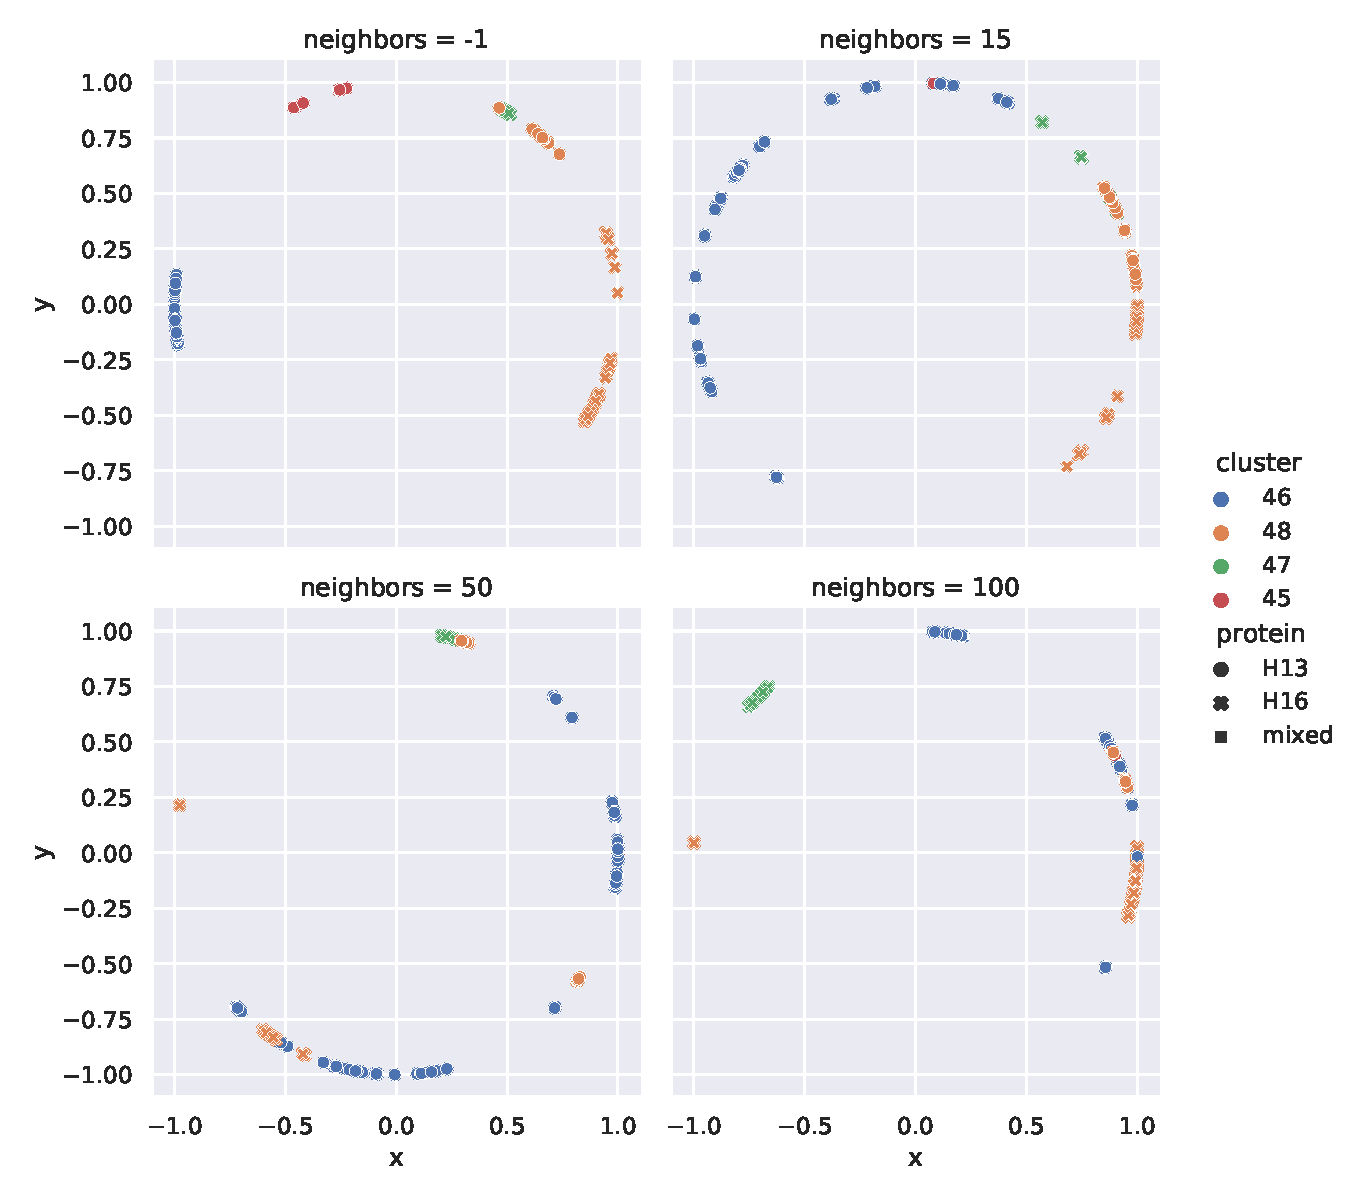
\includegraphics[width=\textwidth]{PCA/Difference_Segment_4_H_metric_cosine.pdf}
    \caption[H13/H16 k-mer frequency vectors component reduction comparison]{\textbf{H13/H16 k-mer frequency vectors component reduction comparison.} The subset of sequences from the H13 and H16 cluster in \autoref{fig:PCA_Clusteree_Knee_4} were reduced down to two dimensions enabling simple visualization. Cluster assignment was preserved from \autoref{fig:PCA_Clusteree_Knee_4} by coloring the points according to it. \texttt{PCA} as well as the combination with \texttt{UMAP} was performed as described in \autoref{sec:Dimension_Reduction} with the lower final dimensionality for visualization. For the combination of \texttt{PCA} and \texttt{UMAP} different values for the neighbors setting were used, the \texttt{UMAP} standard value 15, a average value 50 and the standard value of this project 100. The subtype of the sequences was annotated by different types of points.}
    \label{fig:Reduction_Comparison}
\end{figure}

The visualization of the reduction by \texttt{PCA} is denoted as neighbors value -1 (\autoref{fig:Reduction_Comparison}). It shows five different accumulations of points. Coloring of these points is based on the original clustering example in \autoref{fig:PCA_Cluster_Knee_4}. This is becoming apparent when focusing on the orange cluster 48 points containing H13 and H16 sequences. That way a fundamental distribution on the points of H13 and H16 can be reviewed as well. 
%
%When using the right side as possible indication for clustering, all the points and accumulations of points are very close to each other. Nonetheless a separation with a imagined clustering can be made very easy by building two clusters of the blue points, one of the red and green and three of the orange points. Still, all the points related to H13 would be merged with the orange ones of H16 before the orange H16 points would be merged with the green ones of H16. Thereby the difference between H13 and H16, the higher-ranking goal would be not accomplished because the orange points are so close to each other. 

The reduction with \texttt{PCA} on the subset results in easy separable accumulations of the cluster 46 and 48 points. The distribution of these points is basically in line with the result shown in \autoref{fig:PCA_Cluster_Knee_4}, as their accumulations are well separated, building the two clusters each with the same sequences in both figures. The major difference, however, is the distance between the accumulations of cluster 48 points to each other as well as to the ones of cluster 47. This would probably result in a imaginary clustering of unchanged cluster 46 and 45 and two clusters consisting of the cluster 48 points of which one also contains the points of cluster 47. It seems as if the distance of the cluster 47 points and the H13 cluster 48 points is underestimated to an great extend. By reduction to two dimensions, the difference between cluster 46 and 45 in the \autoref{fig:Reduction_Comparison} (neighbors = -1) picture is preserved and would result as shown in \autoref{fig:PCA_Cluster_Knee_4}, while on the other hand building at least one cluster merging the subtypes. Cluster 47 and 48 are next to each other in \autoref{fig:PCA_Cluster_Knee_4} and would be linked on the next tree-node there.

It appears as if the points of cluster 47 and 48 are possibly quite similar, which is not the case as the \autoref{fig:Precalculated_Cosine} sub trees clearly show the wanted separation of H13 and H16 in cluster 48 as well as the distance to 47. Keeping the lower complexity and the easier reduction of the sequences in this example, through the smaller number of sequences in mind, the consequence of lowering the dimension by \texttt{PCA} to two dimension seems to preserve most of the information related to the difference of cluster 45 and 46. The difference of the subtype separation inside 48 as well as the overall difference to 47 seems to be lost completely. Since the ground truth separation of \autoref{fig:Precalculated_Cosine} seems to be partially present in \autoref{fig:PCA_Cluster_Knee_4}, by at least separating 47 completely from 48, the higher number of dimensions might be in direct connection to the correct separation of some part of H13 and H16. Therefore, the number of components should be increased to the maximum of 50, that still preserves all functions of \texttt{HDBSCAN} for spanning-tree building. 

Comparing these results to the use of \texttt{UMAP} with different settings of the neighbors value, the impact of this parameter becomes clear. The higher the value, the more crowded the points. This explains the behavior in \autoref{subfig:Normalisation_UMAP}. Since a neighbors value of 100 was used as standard, the values are overall crowded in groups of at least 100 points. The random subset for the graphic was reduced by the same setting. The small random sample with a high neighbors value resulted in a low number of overall distribution. The small subset was used with this high standard value to clarify this behavior. Due to the size of the dataset used for the project, a high value for neighbors was used as described in \autoref{sec:Dimension_Reduction}. The same value as well as 15 and 50 neighbors was used on the subset of H13 and H16 segment 4 sequences to visualize the difference. 

None of the settings results in a separation as good as with the sole use of \texttt{PCA}. With the \texttt{UMAP} standard neighbors value of 15 all the points are next to each other and it is difficult to separate them in to clusters. Furthermore, H13 points would be merged with H16 points before merging with others from H13, thereby breaking the subtype division. Still this setting would separate the points somewhat like in \autoref{fig:PCA_Cluster_Knee_4} since no cluster 46 and cluster 48 points were mixed. Setting the neighbors value to 50 results in a spreading of the cluster 46 points and mixing with little islands of cluster 48 points. As mentioned, the color of the points are based on the clustering of \autoref{fig:PCA_Cluster_Knee_4} containing discussed clustering errors, thereby the coloring must not match, since not declared as ground truth. Nonetheless, like with neighbors value 15, the subtypes overlap making separation impossible. With a neighbors value of 100 separation in quite similar clusters as with \texttt{PCA} or as shown in \autoref{fig:PCA_Cluster_Knee_4} would be possible. However, subtype separation was not possible either even when ignoring the cluster 47 points that might be very sensible to the magnitude of preserved information.

%With normalization and without some information seem to be missing necessary to separate the orange points and the green ones. While on the left side the distance was underestimated to an extend making the orange H13 points and the green H16 points collide, the distance on the right side is overestimated, making the subtype distance of the H13 and H16 orange points to small. Since the separation between red and blue, as well as H13 orange and H16 orange is clearer, the method using normalization is still proved to be the better one, in the circumstances that the location of the green points is caused by the low dimension which is proved by \autoref{fig:PCA_Cluster_Knee_4} showing a separation between 47 and 48 and the right method not producing any better results related to the green points. 

In conclusion, the use of PCA gives the best results compared the ones with \texttt{UMAP}. Still there are challenges to overcome as could be seen with the position of the cluster 47 points. Maybe increasing the information preserved by the \texttt{PCA} would give clearer results. This project aimed to find high-quality representations of \gls{IAV} genomes for the purpose or clustering in a extend that was never reached before. Therefore, the usability of \texttt{HDBSCAN} with parameters as good as possible was of higher importance than the use of \texttt{UMAP} at all costs. In the results of the project \texttt{PCA} performed better than \texttt{UMAP} in any case but only with all the tested parameters. Thus, it might be possible to find parameters for \texttt{UMAP} not explored in this project to represent the genomes even better in a equal low dimension in the future.